\normalfalse \difficiletrue \tdifficilefalse
\correctiontrue

%\UPSTIidClasse{11} % 11 sup, 12 spé
%\newcommand{\UPSTIidClasse}{12}

\exer{Barrière Sympact $\star\star$ \label{C2:07:14}}
\setcounter{question}{0}\UPSTIcompetence{C2-07}
\index{Compétence C2-07}
\index{Barrière Sympact}
\ifcorrection
\else
\textbf{Pas de corrigé pour cet exercice.}
\fi

\ifprof
\else
Soit le mécanisme suivant. On a $\vect{AC}=H\vect{j_0}$,  $\vect{CB}=R\vect{i_1}$ et $\vect{AB} = \lambda\vi{2}$. De plus, 
$H=\SI{120}{mm}$ et $R=\SI{40}{mm}$. 

\begin{center}
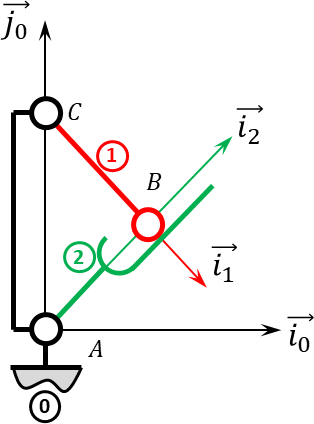
\includegraphics[width=\linewidth]{14_01}
\end{center}
\fi

On néglige la pesanteur sur la pièce \textbf{1}. 

On note $\torseurstat{F}{\text{Moteur}}{1} = \torseurl{\vect{0}}{C_m\vk{0}}{\forall P}$ l'action mécanique du moteur sur la pièce \textbf{1}.

On note $\torseurstat{F}{\text{Ressort}}{2} = \torseurl{\vect{0}}{C_r\vk{0}}{\forall P}$ l'action mécanique d'un ressort couple sur la pièce \textbf{2}. 
%Le raideur du ressort est telle qu'il exerce un couple de \SI{45}{Nm} pour un angle de rotation 100\degres. On considère que le couple est nul lorsque la pièce 2 est à la verticale ($\varphi_o=\dfrac{\pi}{2}$). Il est au maximum lorsque $\varphi_f=0$.

On note $\torseurstat{F}{\text{Pes}}{2} = \torseurl{-Mg\vj{0}}{\vect{0}}{\forall G}$ avec $\vect{AG}=L\vi{2}$. 

\question{Réaliser un graphe d'analyse.}
\ifprof
\begin{center}
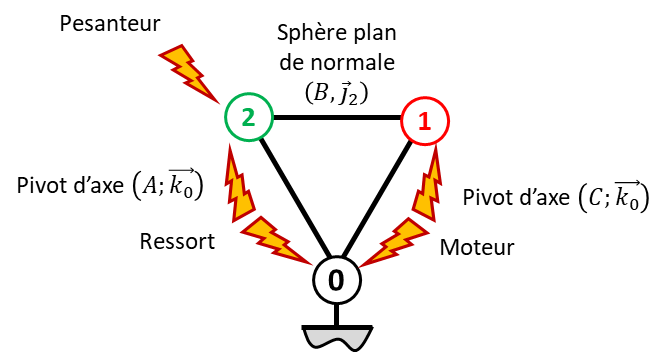
\includegraphics[width=8cm]{14_01_cor}
\end{center}
\else
\fi

\question{Proposer une méthode permettant d'exprimer le couple moteur en fonction des autres actions mécaniques.}
\ifprof
\begin{itemize}
\item On isole 1, on réalise un TMS en $C$ en projection sur $\vect{k_0}$. On obtient une équation liant le couple moteur et l'action normale dans la liaison sphère plan. 
\item On isole 2, on réalise un TMS en $A$ en projection sur $\vect{k_0}$. On obtient une équation liant le couple dans le ressort et l'action normale dans la liaison sphère plan. 
\item En combinant les deux équations on élimine l'action normale dans la liaison sphère plan. On peut éliminer un des deux angles en utilisant la loi entrée sortie.
\end{itemize}
\else
\fi


\question{Mettre en \oe{}uvre une méthode permettant d'exprimer le couple moteur en fonction des autres actions mécaniques.}
\ifprof
\begin{itemize}
\item \textbf{On isole 1.}
\item \textbf{On réalise le bilan des actions mécaniques} : 
\begin{itemize}
\item action de la pivot en $C$ (pas de moment suivant $\vk{0}$),
\item action de la liaison sphère plan en $B$ : $\torseurstat{T}{2}{1} = \torseurl{F_B \vj{2}}{\vect{0}}{B}$, on a alors 
$\babars{C}{B}{2}{1} = R\vi{1}\wedge F_B \vj{2}$
$= RF_B \sin \left(\varphi - \theta + \dfrac{\pi}{2}\right)\vect{k_0}$
$= RF_B \cos \left(\varphi - \theta \right)\vect{k_0}$;
\item $\torseurstat{F}{\text{Moteur}}{1}$.
\end{itemize}
\item \textbf{On réalise le TMS en $C$ en projection sur $\vect{k_0}$} :
$C_m +RF_B \cos \left(\varphi - \theta \right) = 0$.
\end{itemize}


\begin{itemize}
\item \textbf{On isole 2.}
\item \textbf{On réalise le bilan des actions mécaniques} : 
\begin{itemize}
\item action de la pivot en $A$ (pas de moment suivant $\vk{0}$),
\item action de la liaison sphère plan en $B$ : $\torseurstat{T}{1}{2} = \torseurl{-F_B \vj{2}}{\vect{0}}{B}$, on a alors 
$\babars{A}{B}{1}{2} =  \lambda\vi{2}\wedge -F_B \vj{2}$
$=-\lambda F_B \vk{2}$.
\item $\torseurstat{F}{\text{Ressort}}{2}$;
\item action de la pesanteur : 
$\babars{A}{G}{\text{pes}}{2} = L \vi{2} \wedge -Mg \vj{0} $

$= -MgL \sin \left(\dfrac{\pi}{2}-\varphi\right) \vk{0} $

$= -MgL \cos \left(\varphi\right) \vk{0} $

\end{itemize}
\item \textbf{On réalise le TMS en $C$ en projection sur $\vect{k_0}$} :
$C_r-\lambda F_B  -MgL \cos \varphi= 0$.
\end{itemize}

Au final, 
$C_r-\lambda F_B  -MgL \cos \varphi= 0 \Leftrightarrow  F_B  = \dfrac{C_r -MgL \cos \varphi}{\lambda}  $
et
 
$C_m +R \dfrac{C_r -MgL \cos \varphi}{\lambda} \cos \left(\varphi - \theta \right) = 0$.
\else
\fi


\question{Tracer, en utilisant Python, l'évolution du couple moteur en fonction de l'angle de la manivelle. On prendra $M=\SI{1}{kg}$ et $L =\SI{0,1}{m}$}
\ifprof
\url{https://capytale2.ac-paris.fr/web/c/324a-628215/mcer}
\begin{center}
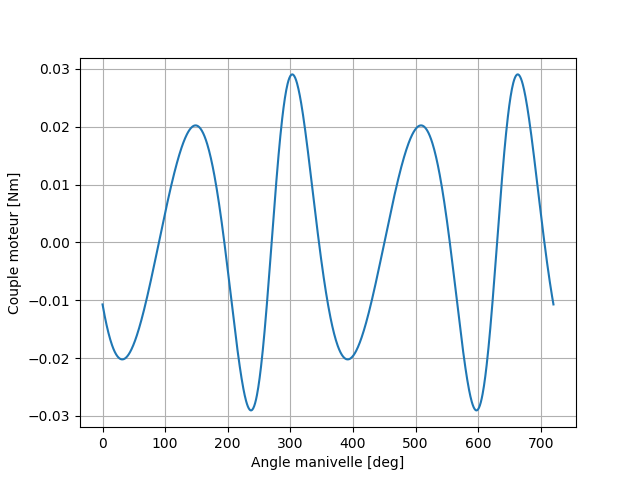
\includegraphics[width=8cm]{14_02_cor}
\end{center}
\else
\fi


\ifprof
\else
\begin{flushright}
\footnotesize{Corrigé  voir \ref{C2:07:14}.}
\end{flushright}%
\fi